\section{Rigid Body Dynamics}

At the heart of the game loop lies the physics engine.
The following section provides an overview of the model for the game world, the movement equations, techniques used for collision detection and resolution, as well as a discussion of the performance.
We also describe problems we encountered and include a comprehensive survey of literature in the area of physics engines for game development.

\subsection{Decoupling of frame rate and physics rate}\label{sec:decoupling}
As mentioned in sec. \ref{sec:gameLoop}, the physics loop is executed one or more times per frame, progressing the simulation in constant time steps $\delta t$.
Having the world state progress at constant speed is good practice as this allows the game to run smoothly and continuously regardless of the varying frame rate (frames per second, $fps$).

We base our implementation on the physics loop proposed by Fiedler \cite{gafferTimestep}.
It uses a time accumulator which \glqq collects\grqq{} the time between the last and the current frame.
The time in the accumulator is then consumed by the physics engine in constant time steps $\delta t$ before the next frame is rendered.
This ensures that no time is lost and even small rest times that were not simulated between frames are accumulated and processed later.

Choosing the $\delta t$ is no trivial manner (c.f. sec. \ref{sec:performance}).
%For our game, choosing $\delta t \in [0.01s, 0.015s]$ yields a pleasant result at a framerate of 60fps.
%One might even choose $\delta t$ bigger than $\frac{1}{\text{fps}}$, the physics simulation then runs at a slower speed than the renderer, which also works but has to be kept in mind.
Because our $\delta t$ is small and the visual benefit is negligible, we deviate from Fiedler's implementation \cite{gafferTimestep} and refrain from interpolating the time residue before rendering.
%This entails undesirable effects like glitching and improper collision resolution (see below).
%Although these effects can be mitigated via interpolation, we received an overall better user experience when running the physics simulation significantly faster than the game loop.
%The reason for this is that collisions that cannot be resolved in a single physics step are resolved before the next frame is rendered.
%On the other hand, if we choose a very small deltaT, we encounter two major problems: the computation of the physics step takes more time than is actually simulated, making the simulation fall behind and if deltaT is very small, rounding off errors might occur.
%Good values that work for up to 30 rocks at the same time when running the game at 60fps lie between 0.1-0.15s.

\vspace{-\abovedisplayskip}
\subsection{The Physics Update}

In one time step of the physics engine, updates are executed in the order depicted in fig. \ref{fig:physicsLoop}.
First, entities and biomes are spawned.
Then, user input events are mapped to world state changes in the Event Processor.
Accelerator and Positioner accelerate entities with gravitational forces and move them accordingly.
During collision handling, collisions between entities are detected and resolved.
This step is performed multiple times to ensure stability of the simulation.
Finally, entities and biomes that are out of scope are destructed.

\vspace{-\abovedisplayskip}
\begin{figure}[h!]
  \centering
  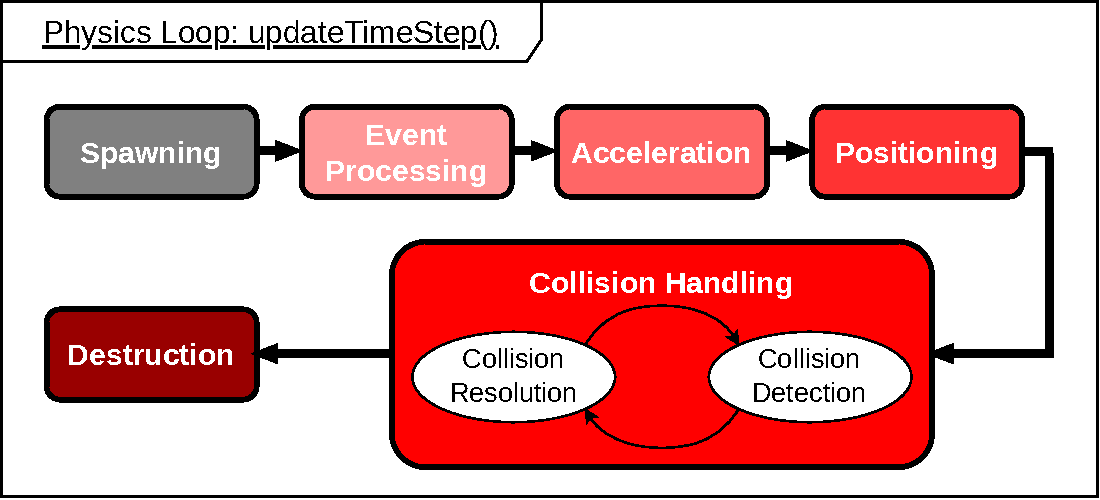
\includegraphics[width = \linewidth]{figures/physics/updateTimeStep.pdf}
  \caption{The physics time step, progressing the world state by $\delta t$. Performed one or more times per frame.}
  \label{fig:physicsLoop}
\end{figure}
\vspace{-\belowdisplayskip}

\subsection{Spawning and Destruction}
The lifetime of entities is managed in the spawning and destruction phase.

\subsubsection{Item and Terrain Generation}

During the spawning phase, items are placed at random positions above the terrain.
The type and frequency of spawned items are configurable.
Furthermore, the biome generation thread is started or joined. %, generating new terrain concurrently once the player approaches the end of the curernt biome.

\subsubsection{Rock Generation}

Rocks are modelled as random convex polygons with a type (e.g. snow/ice/lava/crystal).
The type is chosen randomly with varying probabilities as the game progresses.
It determines a rock's texture and its density $\rho$.

Polygons are obtained by generating a random set of points within a random radius and the subsequent application of Andrew's monotone chain algorithm \cite{polygon_generation}. 
The algorithm determines the convex hull of the set of points as the resulting polygon.
In addition to density, polygons possess mass and a moment of inertia as static properties.
The mass $m$ is defined as the area of the convex polygon times its density $m = \rho A$.
For the moment of inertia $I$, the calculation is based on Fotino's approach \cite{inertia}.
It is illustrated in fig. \ref{fig:inertia}.
The polygon is split into counter clockwise triangles $OV_iV_{i+1}$ with the centroid $O$ constituting the origin.
These triangles are subdivided into right triangles. For the inertia, the following holds:

\vspace{-\abovedisplayskip}
\begin{align}
  I &= \sum_{i=0}^{\#vertices-1} I(OV_{i}V_{i+1 \mod \#vertices})
\end{align}
\begin{align}  
  I(OV_{i}V_{i+1}) &= \alpha_{OV_{i}H_i}\cdot I(OV_{i}H_i) + \alpha_{OH_iV_{i+1}}\cdot I(OH_iV_{i+1}) \nonumber\\
  &= \rho \cdot \Bigg(\alpha_{OV_{i}H_i}\cdot \left(\frac{h_iw_{1,i}^3}{4} + \frac{h_i^3w_{1,i}}{12}\right) \nonumber\\
  &\phantom{= }+ \alpha_{OH_iV_{i+1}}\cdot \left(\frac{h_iw_{2,i}^3}{4} + \frac{h_i^3w_{2,i}}{12}\right)\Bigg)
\end{align}

\noindent $\alpha$ is 1 if a triangle is counter clockwise and -1 otherwise.

After the polygon's static properties are calculated, rocks are spawned at a random position, with random angular momentum, and random linear momentum in x-direction.

\begin{figure}[h!]
  \centering
  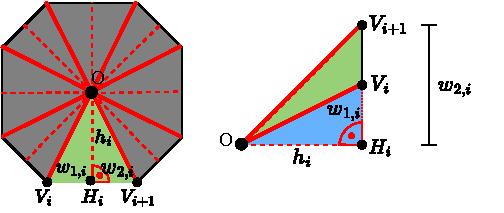
\includegraphics[width = .8\linewidth]{figures/physics/inertia.pdf}
  \caption{The convex polygon is triangulated. The inertia of the polygon is the sum of the inertia of all right subtriangles. On the right, the blue triangle $OV_iH_i$ is clockwise and thus, its inertia has to be subtracted.}
  \label{fig:inertia}
\end{figure}
\vspace{-2\abovedisplayskip}

\subsubsection{Destruction}

Destruction takes place at the end of a physics update.
Rocks that have left the scope of the world or hit the hiker are destroyed and removed.
Similarly, old biomes are destructed.
This garbage collection ensures a consistent performance no matter how long the game runs.  

\vspace{-\abovedisplayskip}
\subsection{Dynamic Properties of Polygons}

The state of a polygon consists of its dynamic properties, i.e. its attributes that may change in every timestep of the physics simulation.
We define a polygon's position $\vec{x} \in \R^{2}$ as the coordinates of its center of mass (centroid).
Its rotation angle around its centroid $\theta \in \R$ is given in radians.
The coordinates of the vertices are stored as body space vertices $\vec{v_i} \in \R^{2}$ in relation to the centroid.
To obtain world space coordinates $\vec{p_i}$ of the vertices, rotation and translation are applied to the body space vertices. 
As the world space vertices are queried often, it has proven beneficial for performance to store the list of world space coordinates of the vertices as a polygon attribute that is recalculated whenever it is moved. 
Furthermore, polygons have a linear momentum $\vec{P} \in \R^{2}$ and an angular momentum $L \in \R$.

\vspace{-\abovedisplayskip}
\subsection{Movement Equations}

Our physics engine is based on impulses and momentum as proposed by Baraff \cite{baraff}.
Since our game is two-dimensional, we are able to reduce his movement equations and receive the following system of partial differential equations:

\begin{align}
  \frac{\textbf{d}}{\textbf{d}{t}} 
  \left(
    \begin{array}{c}
      \vec{x}(t)\\
      \vec{P}(t)\\
      \theta(t)\\
      L(t)
    \end{array}
  \right)
  =
  \left(
    \begin{array}{c}
      {\vec{P}(t)}/{m}\\
      \vec{F}(t)\\
      L(t)/I\\
      \tau(t)
    \end{array}
  \right)
\end{align}
 
We devise a simple, yet effective symplectic Euler solver for this equation:

\begin{align}
  \vec{P}^{t+1} &= \vec{P}^{t} + \delta t \cdot F^{t}\\
  \vec{x}^{t+1} &= \vec{x}^{t} + \delta t \cdot \frac{P^{t+1}}{m}\\
  L^{t+1} &= L^{t} + \delta t \cdot \tau^{t}\\
  \theta^{t+1} &= \theta^{t} + \delta t \cdot \frac{L^{t+1}}{I}
\end{align}

%The simulation works on the dynamic properties of the polygons.
Here, the force $\vec{F}^{t}$ and the torque $\tau^{t}$ are to be read as the sum of all forces or torques applied to a polygon at time step $t$.
A body force only changes the polygon's linear momentum.
In contrast, a surface force $\vec{F}$ applied at a point $\vec{p}$ changes linear and angular momentum.
It generates a torque
\begin{align}
  \tau = (\vec{p} - \vec{x}) \times \vec{F}\label{eq:forceToTorque}
\end{align}
Disregarding collisions, only the gravitational force is considered in our simulation.
It is applied as a body force.

%We define the 2D cross product as
%\begin{align}
%  \left(
%    \begin{array}{c}
%      a\\
%      b
%    \end{array}
%  \right)
%  \times
%  \left(
%    \begin{array}{c}
%      c\\
%      d
%    \end{array}
%  \right)
%  = ac - bd \in \R
%\end{align}

%Put together, the following system of partial differential equations holds for the computation of the movement in two dimensions (c.f. \cite{baraff}):

\subsection{Collision Detection}

After the entities have been moved to their new positions, non-penetration constraints may be violated.
%a check needs to be performed to see whether the new world state is valid.
%In particular, since the simulation assumes perfectly rigid bodies, all collisions must be resolved.
%Therefore, the collision handling algorithm \ref{alg:rockColl} is executed.
Therefore, we check for each rock whether it collides with the player, the terrain or any of the other rocks and resolve it (c.f. sec. \ref{sec:cr}).
Because only pairwise collisions are considered and to ensure stability, this loop is repeated until no collisions occur anymore.
We do however, allow the simulation to stop after a maximum number of resolution steps.
This coincides with our design choice of prioritizing performance over accuracy. 
%
%{
%  \centering
%  \begin{minipage}{\linewidth}
%    \vspace{-\abovedisplayskip}
%    \begin{algorithm}[H]
%    \caption{Rock Collision Handling}\label{alg:rockColl}
%    \textbf{Input:} rocks: list(Rock)
%      \begin{algorithmic}[1]
%      \Procedure{handleCollisions}{rocks, maxSteps$=4$}
%      \State resolutionSteps $\gets$ 0
%      \Repeat
%        \ForAll{rock : rocks}
%          \State terrainCollision(rock)
%          \State playerRockCollision(rock)
%          \ForAll{otherRock : rocks}
%            \State rockCollision(rock, otherRock)
%          \EndFor
%          \State resolutionSteps++
%        \EndFor
%      \Until{noCollisions $\lor$ resolutionSteps = maxSteps}
%      \EndProcedure
%      \end{algorithmic}
%    \end{algorithm}
%  \end{minipage}
%}
%\vspace{\belowdisplayskip}

\subsubsection{Separating Axis Theorem}

There are many options for collision detection between convex polygons, such as the Gilbert-Johnnson-Keerthi algorithm (GJK) \cite{GJK}, Minkowski Portal Refinement (MPR) \cite{gemsMPR} and different variations of the separating axis theorem (SAT) \cite{geometrySAT}.
For the sake of simplicity and efficiency, we chose an SAT based approach.
The SAT states that two convex polygons do not collide if and only if there exists a separating axis.
If a separating axis exists, a separating axis can be found that is parallel to one of the polygons' edges.
Fig. \ref{fig:SAT} demonstrates this with an example.
Our implementation of the SAT roughly follows the algorithms outlined by Wheeler \cite{wheelerCD}.
Separating axes are found by projecting all vertices of both polygons on all edge normals.
If a separating axis is found, the algorithm instantly returns.
Otherwise, if none of the edges constitutes a separating axis, the edge with the smallest overlap of the projections is returned.
This edge is called the reference edge and the corresponding polygon is called \emph{reference polygon}.
The other polygon is the \emph{incident polygon}.

\subsubsection{Optimizations}\label{sec:opt}

We take measures to increase the performance of our collision detection routines.
When a separating axis to another polygon is found, its index is stored in a map accessed by a polygon ID.
When those two polygons are checked for collisions the next time, the detection algorithm starts with this edge as there is a high probability that it is a separating axis again and the algorithm can return early.
This concept is called \emph{warm starting}.

Moreover, we use \emph{swept axis-aligned bounding boxes} (swept AABBs) \cite{sweptAABB, tutorial} (see fig. \ref{fig:aabb}).
The rather expensive SAT algorithm is not executed when the swept AABBs do not collide.
In addition to increasing performance, the use of swept AABBs also increases accuracy.
If a potential collision is signalled by the AABB check, the last simulation step is substepped if the rocks are \glqq fast\grqq{}, i.e. the following holds for the two velocities $\vec{v_1} = \vec{P_1}/m_1$ and $\vec{v_2} =  \vec{P_2}/m_2$:
\begin{equation}
  \norm{\vec{v_1}} + \norm{\vec{v_2}} > \frac{\text{minPolySize}}{2\delta t} 
\end{equation}
We approximate continuous collision detection by using a small but constant $\delta t' < \delta t$ for substepping.
In order to ensure efficient access, the swept AABB is calculated and stored during positioning.
Furthermore, to allow local substepping via interpolation, the last position $\vec{x}^{t-1}$ and rotation angle $\theta^{t-1}$ are kept as attributes.

\begin{figure}[htbp]
  \centering
  \begin{minipage}{.53\linewidth}
    \centering
    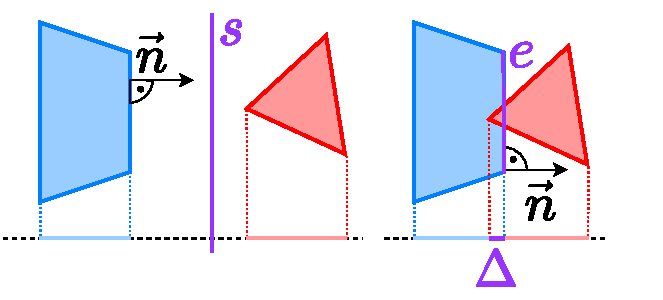
\includegraphics[width=1.09\linewidth]{figures/physics/sat.pdf}
    \caption{SAT: On the left, the separating axis is $s$. On the right, no separating axis exists, the algorithm returns the reference edge $e$, which has the smallest collision depth $\Delta$.}
    \label{fig:SAT}
  \end{minipage}\hspace{.04\linewidth}%
  \begin{minipage}{.43\linewidth}
    \centering
    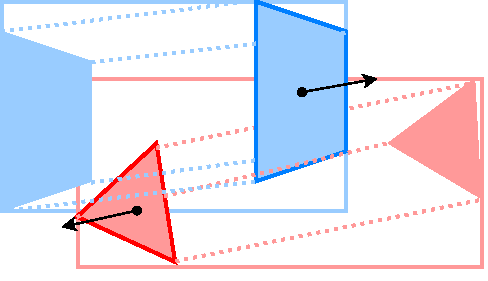
\includegraphics[width=\linewidth]{figures/physics/aabb.pdf}
    \caption{Swept AABBs increase accuracy. Potential collisions can be detected even if the objects are not currently colliding.}
    \label{fig:aabb}
  \end{minipage}
\end{figure}
\vspace{-\abovedisplayskip}

\subsubsection{The Terrain}\label{sec:terrainCD}

By itself, the SAT only works for convex polygons.
However, our terrain is concave.
To handle this with our existing collision detection architecture, we triangulate the terrain using the poly2tri library's constrained Delaunay triangulation \cite{poly2tri}.
Using triangles, all the collision detection methods above work as is.
We still need to retrieve the relevant parts $T_{cd}$ of the terrain and create a polygon as input for poly2tri from the line representation of the terrain.
%In contrast to rocks, this polygon is not necessarily convex, as the terrain itself is not convex.

In order to achieve this, we first compare the swept axis aligned bounding box $AABB_e$ of the entity with the axis aligned bounding boxes $AABB_{t_{i}}$ of the terrain sections $T_{i, cd}$. 
Here, we filter out the sections $T_{min, cd}$ and $T_{max, cd}$ as the first and last terrain sections $T_{i, cd}$ for which $AABB_{t_{i}}$ overlaps with $AABB_e$.
Then, we create a new polyline $Pl_{T,e}$ by combining all sections from $T_{min, cd}$ to $T_{max, cd}$ along the terrain:
\begin{align}
  Pl_{T,e} = (T_{min, cd}, T_{min + 1, cd}, \dots, T_{max - 1, cd}, T_{max, cd})
\end{align}

After that, we combine the hitboxes $AABB_e$ of the entity and $AABB_{PL_{T,e}}$ of the created polyline into a merged $AABB_{e, PL_{T,e}}$ that includes both of them and has an additional tolerance to each side.
Then, we project the first and last point of $Pl_{T,e}$ outwards onto $AABB_{e, PL_{T,e}}$ and add those points $p_{min}$ and $p_{max}$ to the start and end of $Pl_{T,e}$.
As a last step, we close the modified Polyline to a polygon $P_{T,e}$ by adding the corners $c_{min}, c_{min+1}, \dots, c_{max}$ of $AABB_{e, PL_{T,e}}$ in between $p_{max}$ and $p_{min}$ in clockwise order.

\vspace{-\abovedisplayskip}
%need the hitboxes $AABB_e$ of the entity and $AABB_{PL_{T,e}}$ of the created polyline. 
%We merge these bounding boxes into one bounding box $AABB_{e, PL_{T,e}}$ that includes both of them and has an additional tolerance to each side.
%Additionally, we compute which of the four edges of $AABB_e$ $T_{min, cd}$ and $T_{max, cd}$ intersect with. Then, we project the first point of $T_{min, cd}$ and the last point of $T_{max, cd}$ outwards to the corresponding edges of $AABB_{e, PL_{T,e}}$. 
%This process yields two new points $p_{min}$ and $p_{max}$ which are added to the start and end of $PL_{T,e}$ respectively to form $PL'_{T,e}$.

%As a last step, we add corners $c_{min}, c_{min+1}, \dots, c_{max}$ of $AABB_{e, PL_{T,e}}$ to the end of $PL'_{T,e}$ that are between $p_{max}$ and $p_{min}$ when traversing $AABB_{e, PL_{T,e}}$ in clockwise order from $p_{max}$ to $p_{min}$.
%This forms the final polygon $P_{T,e}$:
\begin{align}
 P_{T,e} = \:& (p_{min}, T_{min, cd}, T_{min + 1, cd}, \dots, T_{max, cd},\notag\\
 & \quad p_{max}, c_{min}, c_{min + 1} \dots, c_{max})
\end{align}

The process of creating such a polygon for both normal terrain and in case of overhangs is illustrated in fig. \ref{fig:terrainCollisionPoly}.

\imagewithwidth{figures/TerrainCollisionPoly.pdf}{\columnwidth}{fig:terrainCollisionPoly}{Creating a polygon from relevant terrain sections for collision detection and collision handling with rocks.  Here shown for normal terrain and overhang.}{}
\vspace{-3\abovedisplayskip}

\subsection{Collision Resolution}\label{sec:cr}

When a collision between two polygons is detected, the colliding objects are displaced to restore the validity of the current world state.
Additionally, appropriate reactive impulses are applied.

\begin{figure}[h!]
  \centering
  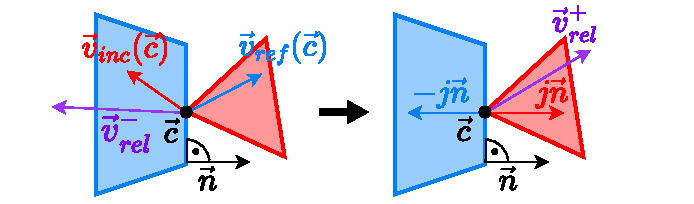
\includegraphics[width = .8\linewidth]{figures/physics/resolution.pdf}
  \caption{On the left, the polygons have been displaced to their first point of collision. $\vec{v}_{rel}^{\,-}$ is opposed to $\vec{n}$. The right side shows how the collision is resolved by applying impulses $\pm j\vec{n}$, so that $\vec{v}_{rel}^{\,+}$ is no longer opposed to $\vec{n}$.}
  \label{fig:CR}
\end{figure}

\vspace{-\abovedisplayskip}
\subsubsection{Displacement}

In addition to transferring the world back to a valid state, displacement serves the purpose of approximating the first point of contact between two objects.
Only there, impulses can be applied accurately.
Once a collision occurs, the colliding polygons are moved apart by the collision depth $\Delta$ along the collision normal.
We weigh the displacement by mass to increase stability \cite{wheelerCD}.
\begin{align}
  \vec{x}_{ref}^{\,+} &= \vec{x}_{ref}^{\,-} + \Delta \cdot \frac{m_{ref}}{m_{ref} + m_{inc}} \cdot (1+\epsilon)\\
  \vec{x}_{inc}^{\,+} &= \vec{x}_{inc}^{\,-} + \Delta \cdot \frac{m_{inc}}{m_{ref} + m_{inc}} \cdot (1+\epsilon)
\end{align}
The superscripts $^-$ and $^+$ denote the state before and after collision resolution.
A small $\epsilon$ is introduced here and in eq. \ref{eq:vrel} to ensure stability.

If the collision was found by substepping, we first set the polygons to their positions at the time of the collision substep and then apply displacement from there. 

\subsubsection{Impulse Application}

Not every contact is necessarily a collision.
Only when rocks are moving towards one another at a contact point, we consider it a collision requiring the application of impulses.
Fig. \ref{fig:CR} shows that this is the case, when the relative velocity $\vec{v}_{rel}$ at the contact point $\vec{c}$ is opposed to the normal $\vec{n}$, i.e.:
\begin{align}
  \left<\vec{n},\vec{v_{rel}}\right> = \left<\vec{n},\vec{v_{inc}}(\vec{c})-\vec{v_{ref}}(\vec{c})\right> < -\epsilon\label{eq:vrel}
\end{align}
where
\begin{align}
  \vec{v}(\vec{c}) = \frac{\vec{P}}{m} + \frac{L}{I}
  \left(\begin{array}{c c}
    0 & -1\\
    1 & 0
  \end{array}\right)
  (\vec{c} - \vec{x})
\end{align}
Finally, the impulse is applied to both the incident and the reference polygon.
The formula for the magnitude $j$ of the impulse has been derived by Baraff \cite{baraff}:
\begin{align}
  j = \frac{-(1 + \gamma)\left<\vec{n},\vec{v_{rel}}\right>}{\Theta_{inc} + \Theta_{ref}}\label{eq:scary}
\end{align}
with 
\begin{align}
  \Theta = \frac{1}{m} + \left<\vec{n},\left(\frac{1}{I}((\vec{c} - \vec{x})\times \vec{n})\right)\times (\vec{c} - \vec{x})\right>
\end{align}
$\gamma \in [0, 1]$ is the coefficient of restitution.
Intuitively, it describes how much of the impulse is preserved and how \glqq bouncy\grqq{} a collision is.
The resulting impulse is applied as a surface force $-j\vec{n}$ for the reference polygon and $j\vec{n}$ for the incident polygon at the contact point $\vec{c}$.
% Potentially remove
This force also generates a torque (see equation \ref{eq:forceToTorque}).
The polygon experiences an instantaneous change in linear and angular momentum.

For terrain collisions, impulse and displacement are evidently only applied to the polygon and not on the terrain triangles which are static.

\subsection{Beyond Rock Collisions}

So far, we only discussed convex polygons.
The algorithms as described above can be applied to rocks without restriction.
The hiker behaves very similarly but with some key differences.
The hiker movement is governed by the user input.
Gravity is only applied when the hiker is in the air. 
For collisions, the hiker hitbox is a convex polygon that does not rotate.
When a rock hits the hiker, the rock is destroyed and damage is applied to the hiker.
Moreover, a knockback impulse based on the rock's impulse is applied to the hiker.

Terrain collisions are also different.
In air, the hiker bounces off the terrain like a rock would.
On the ground however, the hiker needs to be able to walk smoothly without colliding with the terrain.
This is achieved by clamping the hiker on the terrain with a small upward displacement $(0, \epsilon)^T$, so that the hiker only collides with overhangs and walls and not the terrain below.
Further checks were implemented e.g., to guarantee that the hiker cannot climb or descend a slope that is too steep.

The most simple entity is the monster or kill bar.
Its movement is only characterized by an x coordinate.
\begin{align}
  x_{\text{monster}}^{t+1} = x_{\text{monster}}^{t} + \delta t \cdot v_{\text{monster}}^{t}
\end{align}
The texture is always placed on top of the terrain.
With the velocity of the monster increasing over time, difficulty is raised.
There are no collisions with the monster.

\subsection{Performance Aspects}\label{sec:performance}

This section supplements the optimizations introduced in sec. \ref{sec:opt} with performance analytics.
Thorough scrutiny of the performance of our physics engine is paramount for the game to run smoothly seeing as the physics update is the most important and - if there are many entities - expensive part of the game loop.
%In contrast to the terrain generation, this part can only be parallelized with great effort, which is why we attempted to increase performance of the sequential execution of physics updates between frames.

Our physics engine can simulate a heap of up to 50 rocks (a heap is the worst case scenario as rocks are constantly colliding).
With the right configuration of the physics engine, the simulation can be pushed to up to 100 rocks, however, some visual accuracy and smoothness is lost.
The crucial parameters for the performance of the physics engine are $\delta t$ and the maximum number of physics steps added to the accumulator (c.f. sec. \ref{sec:decoupling}) per frame.
The latter presents a solution for what Fiedler \cite{gafferTimestep} calls the \glqq spiral of death\grqq{}.
This phenomenon occurs when the physics engine takes more time to consume the time in the accumulator than the time currently in the accumulator.
In that case, more time is added to the accumulator than in the previous step, effectively dropping the frame rate to zero after a while.
By limiting the maximum number of physics steps that are added to the accumulator per frame ($spf$), this effect can be mitigated to a certain degree.
Fig. \ref{fig:perf} shows the effects of these parameters on a compute-heavy simulation with many rocks.

%Interestingly, the choice of $\delta t$ has only a minor effect on performance.
A larger $\delta t$ leaves more room for the physics engine update step and thus the $fps$ drop a bit later.
However, the choice of the $spf$ seems far more important. 
Using an $spf>2$ we always run into a spiral of death during the simulation.
In the actual game however, we even use $spf=10$ (and $\delta t=0.015s$).
This is because in a real game, the number of rocks is much smaller, so performance is not an issue.
The choice of a bigger $spf$ yields visually smoother and more accurate results.
%Although the effect of $spf$ on $fps$ is obvious, we can only speculate why $spf$ has an impact on the time needed for a physics update.
%We assume that this effect stems from stack management overhead when more steps are performed per frame.

\begin{figure}[h!]
  \centering
  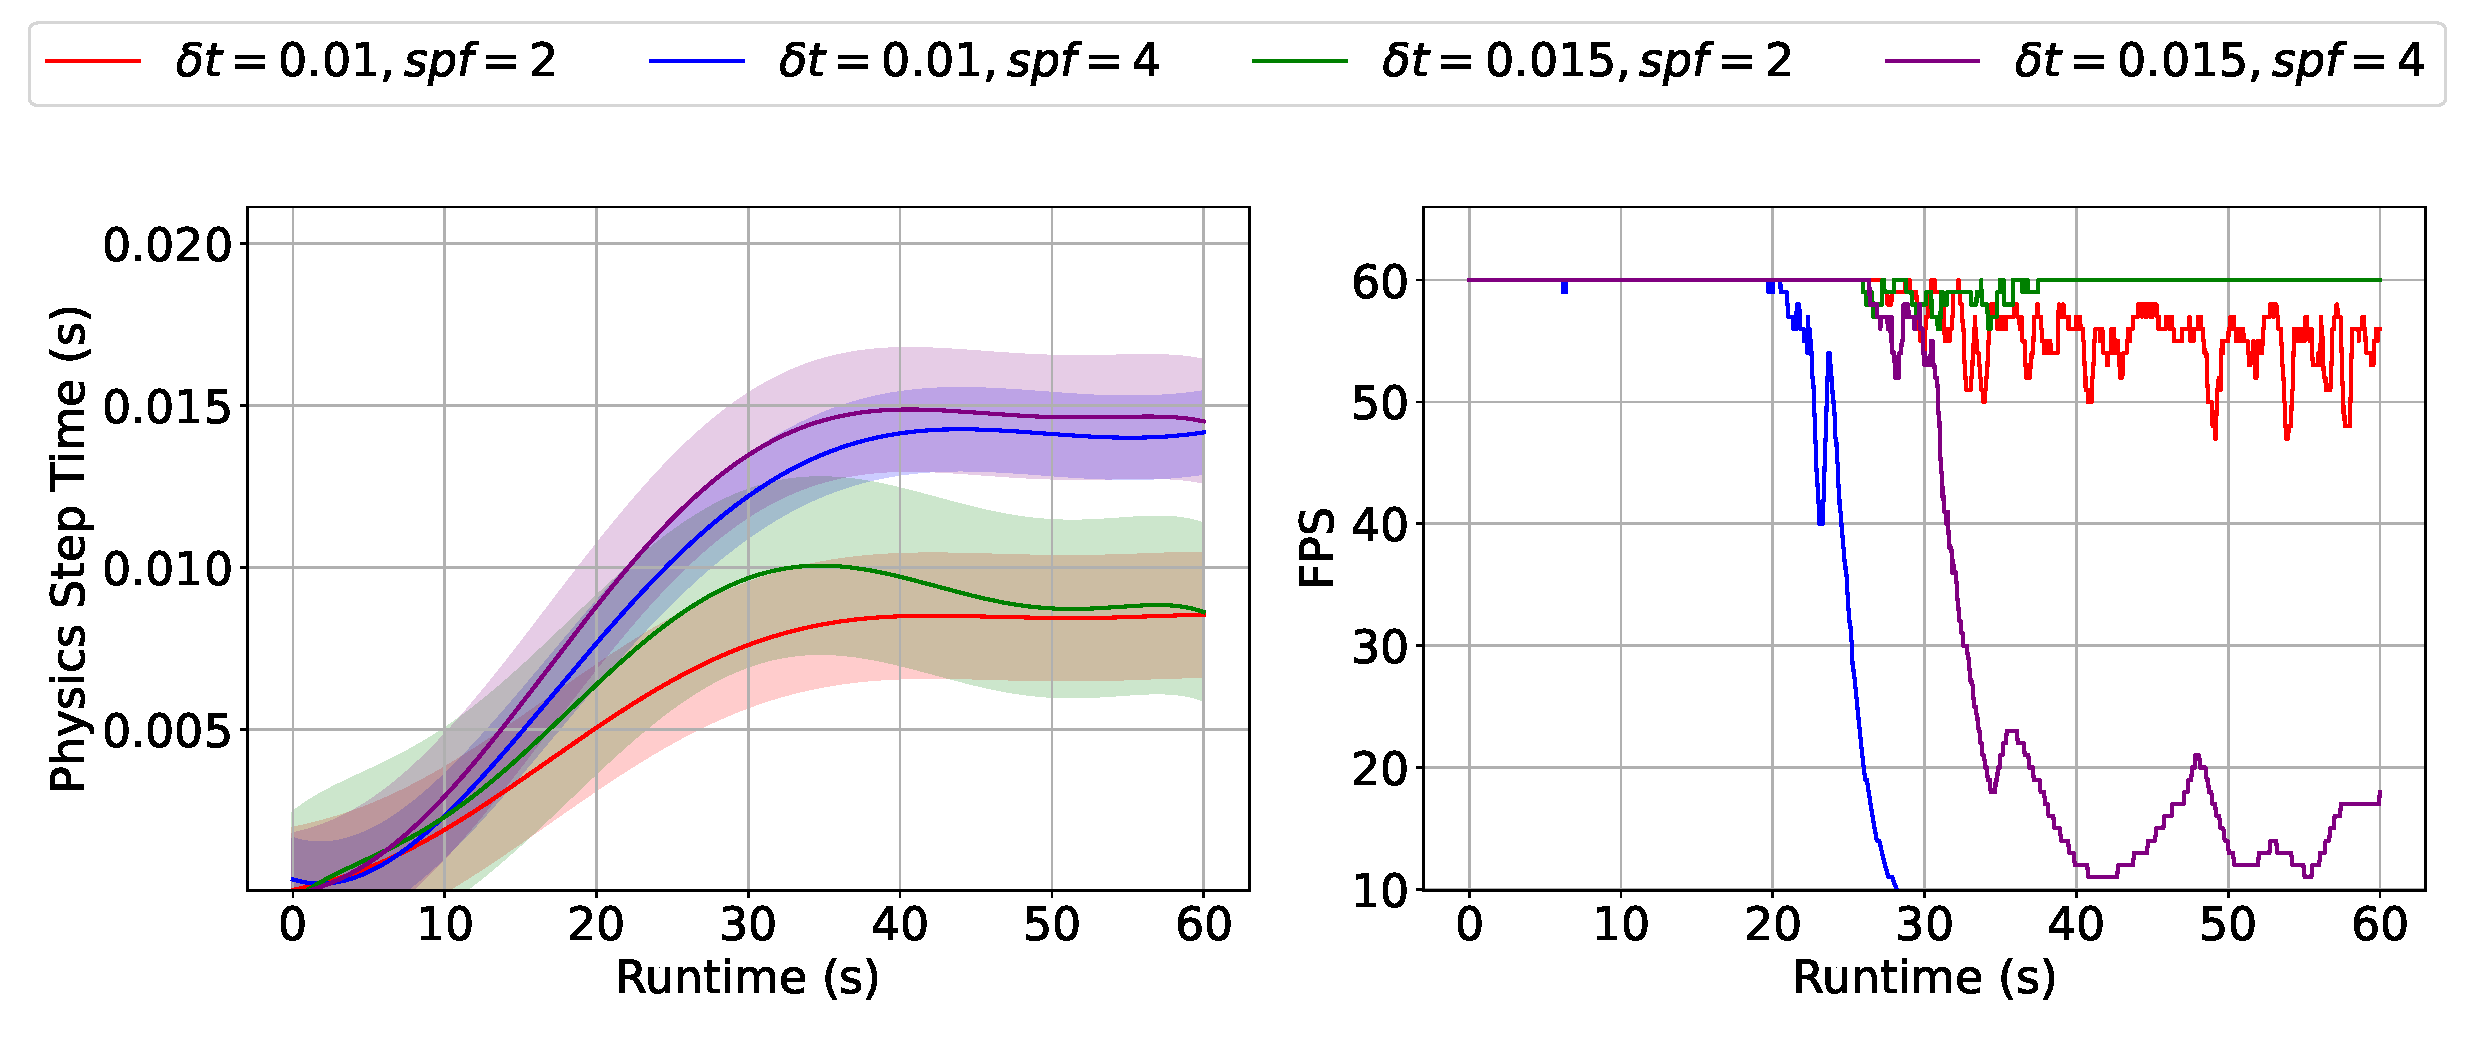
\includegraphics[width = \linewidth]{figures/physics/perf.pdf}
  \caption{Time needed for a physics update (left) and frame rate (right) over the course of a simulation dropping 100 rocks into a bowl in the first 30s. The physics update times are approximated via regression using polynomials of degree 6 and a 95\% confidence bound is plotted. For $spf=4$, we run into the spiral of death.}
  \label{fig:perf}
\end{figure}

In conclusion, although it is not arbitrary scalable, we deem the performance of the physics engine sufficient for the purpose of our game.
Using efficient garbage collection when entities and terrain leave the scope of the game in combination with adequate performance allows the game to always run steadily.

